\section{Improving a baseline quoting policy under uncertainty}
\label{sec:baselinequoting}

The preceding certificates bound loss relative to a model-specific optimum.
A different deployment question compares a candidate with the policy already
running. Baseline-relative robust policy improvement is established by
\citet{GhavamzadehPetrikChow2016}. Here its continuous-time specialization
uses the tagged queue state, a supplied enclosure of the baseline value,
and an explicit lower bound on the improvement. It does not require the
unknown optimal value or an online exploration claim.

\subsection{An advantage measured against one common law}

Fix a finite state and action space, discount $\beta>0$, and a family
$\theta\in\Theta$ of bounded reward rates $r^{a,\theta}$ and generators
$L^{a,\theta}$. The state includes every outstanding reservation and any
pending cancellation. Let $b(x)$ be a stationary baseline and
\[
 V^{b,\theta}=(\beta I-L^{b,\theta})^{-1}r^{b,\theta}.
\]
Suppose vectors $l,u$ satisfy $l\le V^{b,\theta}\le u$ for every $\theta$.
For a row difference $D_{xy}^{a,\theta}=L_{xy}^{a,\theta}-L_{xy}^{b,\theta}$,
define
\begin{align}
 \underline A_x(a)=\inf_{\theta\in\Theta}\bigg\{
 r_x^{a,\theta}-r_x^{b,\theta}
 +\sum_{y:D_{xy}^{a,\theta}\ge0}D_{xy}^{a,\theta}l_y
 +\sum_{y:D_{xy}^{a,\theta}<0}D_{xy}^{a,\theta}u_y\bigg\}.
 \label{eq:baselineadvantage}
\end{align}
This is the exact minimum over the supplied value rectangle and the
parameter family; the rectangle can be an enlargement of the attainable
baseline values. The baseline action has $\underline A_x(b(x))=0$ exactly.
The same $\theta$ must be used in both terms of each reward and generator
difference. Separately minimizing the candidate and maximizing the baseline
can destroy cancellations and make the bound needlessly pessimistic.

\begin{theorem}[A certified baseline policy improvement]
\label{thm:baselinequoting}
Choose a stationary policy $\pi$ with $g_x:=\underline A_x(\pi(x))\ge0$
for every state, retaining $b(x)$ when no strictly positive alternative is
certified. Then, for every $\theta\in\Theta$,
\begin{equation}\label{eq:baselinegain}
 V^{\pi,\theta}-V^{b,\theta}
 \ge (\beta I-L^{\pi,\theta})^{-1}g\ge0.
\end{equation}
Any vector $z$ satisfying
\begin{equation}\label{eq:baselinegainsubsolution}
 \beta z_x\le g_x+\inf_{\theta\in\Theta}(L^{\pi,\theta}z)_x
\end{equation}
is a simultaneous lower bound on this value improvement.
With a common exit-rate bound $\Lambda$, start $z^0=0$ and iterate
\begin{equation}\label{eq:baselinegainiteration}
 z^{k+1}_x=
 \frac{g_x+\Lambda z^k_x+
          \inf_{\theta\in\Theta}(L^{\pi,\theta}z^k)_x}{\beta+\Lambda}.
\end{equation}
Each iterate is a lower bound. Downward rounding preserves the bound;
replacing a negative rounded coordinate by zero also preserves it.
\end{theorem}
\begin{proof}
Under one fixed law, the baseline advantage is
$A^{\pi,b,\theta}=r^{\pi,\theta}-r^{b,\theta}
 +(L^{\pi,\theta}-L^{b,\theta})V^{b,\theta}$.
Subtract the two policy equations to obtain the exact identity
\[
 (\beta I-L^{\pi,\theta})(V^{\pi,\theta}-V^{b,\theta})
       =A^{\pi,b,\theta}.
\]
Minimizing a linear form over $[l,u]$ proves $A^{\pi,b,\theta}\ge g$.
The resolvent is the integral of a positive discounted transition
semigroup, proving \eqref{eq:baselinegain}. Multiplying the subsolution
inequality by this positive resolvent proves its assertion. Uniformization
makes the iteration monotone, with contraction factor
$\Lambda/(\beta+\Lambda)$. It lies below each model's fixed-policy map
with reward $g$. Starting at zero and induction therefore bound its value,
including downward rounding. Nonnegativity permits clipping a rounded lower
bound at zero. Combining these facts proves the finite-iterate statement.
\end{proof}

\begin{remark}[Policy value, not realized pathwise profit]
The comparison is between discounted expectations from every modeled state.
It does not imply that every realized trading path improves, that withdrawal
liquidates inventory, or that a nominally safe action remains safe after the
law leaves $\Theta$. Rectangular enlargement is allowed when computing a
lower bound for a fixed parameter family. It need not represent a single
law attaining every rowwise infimum. All actions must share valid physical
state transitions, including executable orders during cancellation latency.
\end{remark}

\subsection{The message-clock specialization}

In the replacement-clock model the external events are common to the
messages at a given state. A message $a$ sends $x$ to $R_a(x)$ at known
rate $\nu$ and costs $c_x(a)$. Write $y=R_a(x)$ and $z=R_{b(x)}(x)$.
External rewards, external generators, and the diagonal clock term cancel.
Consequently a computable lower advantage is
\begin{equation}\label{eq:messagebaselinegain}
 \underline A_x(a)=\nu\left[
 \begin{cases}l_y-u_z,&y\ne z,\\0,&y=z\end{cases}
 -c_x(a)+c_x(b(x))\right].
\end{equation}
When destinations agree their value difference is exactly zero, regardless
of the enclosure width. This cancellation is particularly useful when two
message labels induce the same physical transition.

The bounds $[l,u]$ must enclose the \emph{baseline} value, not the optimal
value from Theorem~\ref{thm:intervalcontrol}. They are obtained by fixing the
message $b(x)$ in that theorem's lower and upper uniformized recursions.
The same monotonicity proof applies. An independent alternative starts
from a computed baseline value $v$. If
\[
 \sup_{x,\theta}|r_x^{b,\theta}
                     +(L^{b,\theta}v)_x-\beta v_x|\le\eta,
\]
then $v-\eta\mathbf1/\beta\le V^{b,\theta}
\le v+\eta\mathbf1/\beta$ by the resolvent norm bound. This accounts
for both model discrepancy and a numerical policy-evaluation residual.

\begin{corollary}[Randomization, repeated improvement, and tolerance]
Any statewise mixture supported on actions with nonnegative certified
advantage also improves on $b$. A finite succession of such improvements,
each with a fresh valid enclosure for its new baseline and the same family
$\Theta$, is monotone in value for every $\theta\in\Theta$.
If numerical errors are bounded by $e_x(a)$, replace an approximate
advantage by its certified lower endpoint before screening actions.
\end{corollary}
\begin{proof}
Rewards and generators are affine in statewise action probabilities, so
the advantage is the corresponding convex combination. Apply the theorem
and then transitivity to successive baseline comparisons. Certified lower
endpoints preserve the required nonnegativity.
\end{proof}

Repeated improvement need not reach a globally optimal policy. A wide
enclosure can block every nontrivial change; this is a meaningful output.
Nor does choosing actions greedily with an estimated baseline value alone
provide this guarantee. Near a switching boundary even a small value error
can reverse a message comparison.

\subsection{A queue-aware baseline experiment}

The experiment reuses the 74 states and all admissible messages of
Section~\ref{sec:intervalexample}. The nominal optimum is used to construct the baseline.
That baseline deliberately discards tagged rank: at a back-of-queue state,
it applies the action chosen at the otherwise identical front state.
This reproduces a concrete information omission, not an arbitrarily poor
constant policy. For each uncertainty multiplier the script computes
320 lower and upper baseline-value iterations with exact fractions and
12-decimal outward rounding. It evaluates all admissible messages and accepts positive certified
changes and computes 320 lower-gain iterations.

\begin{table}[htbp]
\centering
\caption{Synthetic queue experiment. Gains are discounted model objective
units from the empty, zero-inventory state in regime zero. The lower bound
covers the entire stated box; the last column is a nominal-model evaluation.}
\label{tab:baselinequoting}
\begin{tabular}{rrrr}
\toprule
Uncertainty & Changed states & Certified gain & Nominal gain\\
\midrule
\inputtable{tables/certified_improvement_rows.tex}
\bottomrule
\end{tabular}
\end{table}

\begin{figure}[htbp]
\centering
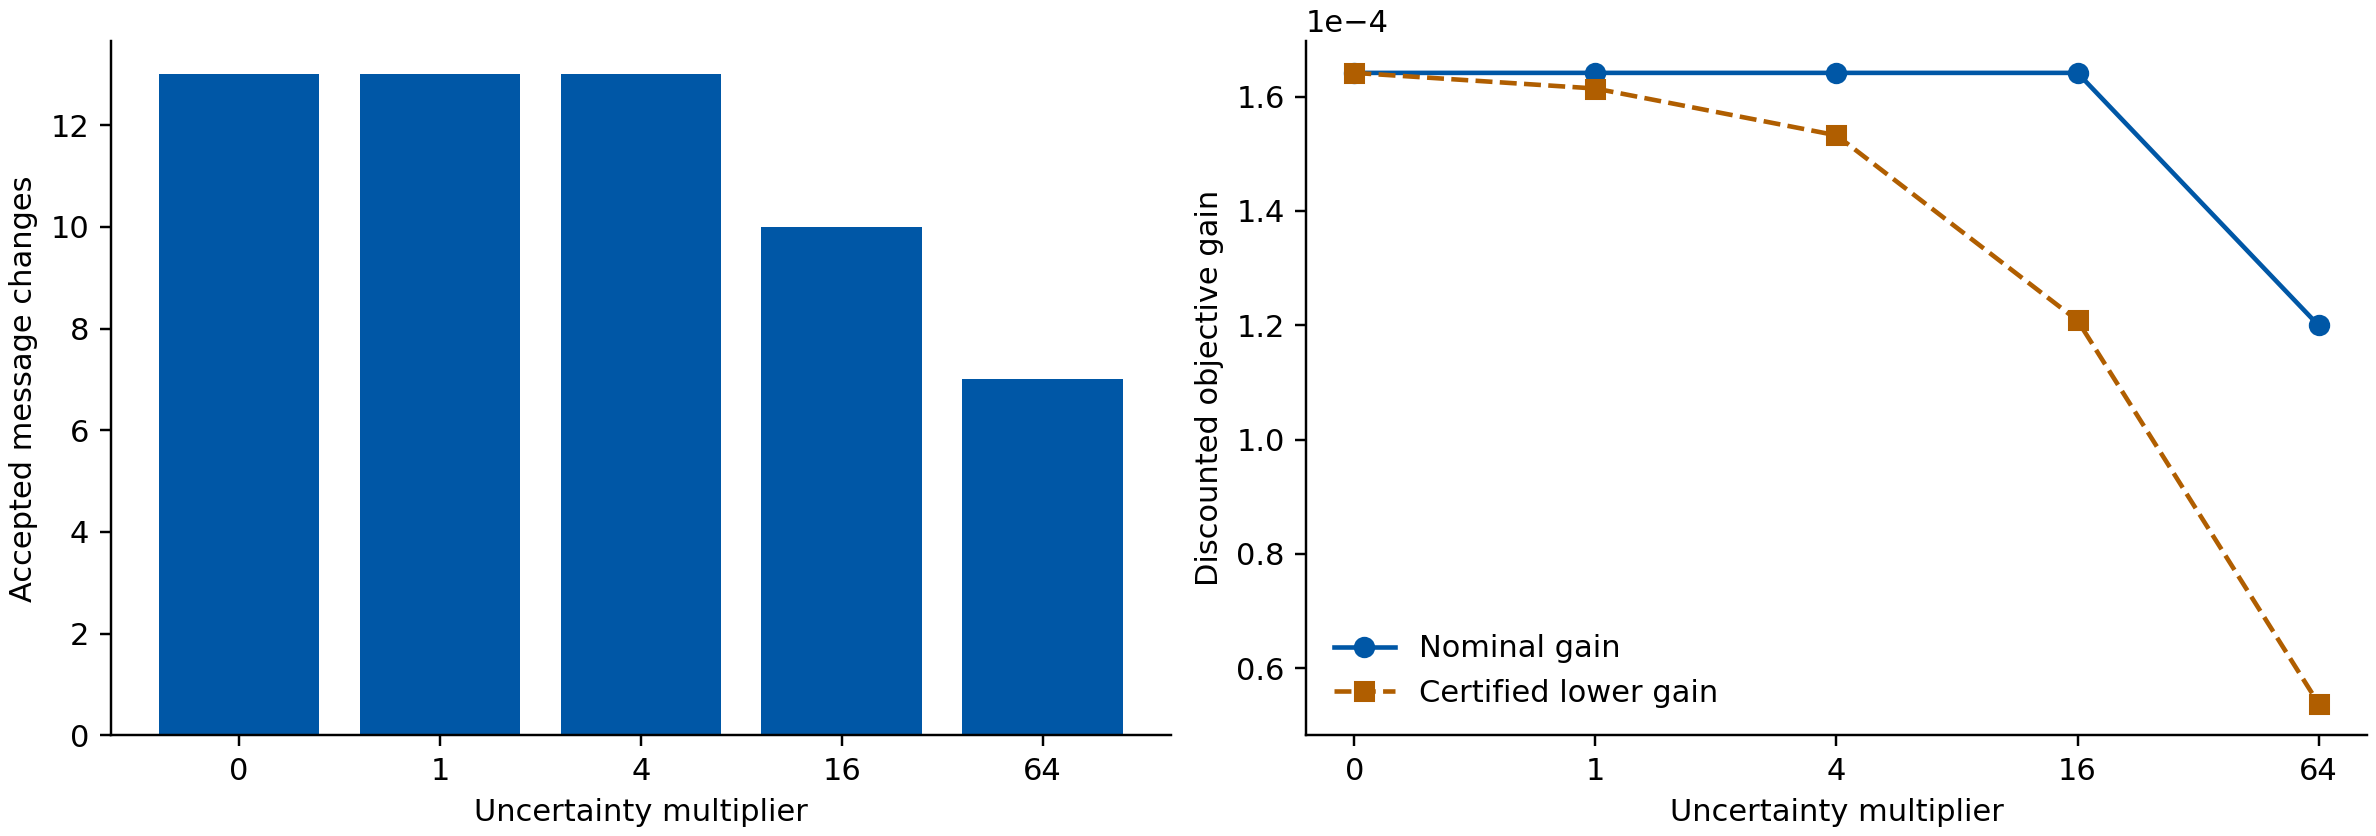
\includegraphics[width=0.94\linewidth]{figures/06_certified_improvement.png}
\caption{A baseline policy can be improved selectively as queue-law
uncertainty changes. Certified gains use rational outward enclosures;
nominal gains use independent linear policy evaluation. The plotted
experiment is synthetic and excludes empirical profitability claims.}
\end{figure}

The script \texttt{verification/certified\_improvement.py} independently
evaluates both policies by solving their linear systems at the center,
at aligned lower and upper corners, and at 20 seeded, independently varied
event-law draws. It verifies the exact performance-difference identity and
the lower-gain comparison in every state. These sampled comparisons are
diagnostics; coverage of the whole box comes from the proved enclosure
and rational arithmetic, not from sampling. A zero-uncertainty comparison
also tests the contraction remainder rather than silently treating a
finite iteration as an exact fixed point.

To turn this into market evidence, log receipt, decision, send, acknowledgement,
fill and cancellation times, and retain an order's tagged priority or its
identifiable bounds. Estimate state- and action-conditional event laws on
training days, freeze the baseline and screened policy, and report acceptance
frequency together with held-out inventory, markout, fees and net P\&L.
Off-policy logs without coverage cannot identify counterfactual fills;
the screening theorem does not repair that identification problem.
